%===============================================================================
% $Id: ifacconf.tex 19 2011-10-27 09:32:13Z jpuente $  
% Template for IFAC meeting papers
% Copyright (c) 2007-2008 International Federation of Automatic Control
%===============================================================================
\documentclass{ifacconf}

\usepackage{graphicx}      % include this line if your document contains figures
\usepackage{natbib}        % required for bibliography


\usepackage[T1]{fontenc}
\usepackage[utf8]{inputenc}

% source code listing
\usepackage{listings}
%\usepackage{minted} % some extra configuration an libraries would be necessary

% configure listings
\lstset{numbers=left,                   % where to put the line-numbers
	numberstyle=\footnotesize,          % the size of the fonts that are used for the line-numbers
	stepnumber=1,                   % the step between two line-numbers.
	numbersep=5pt,                  % how far the line-numbers are from the code
	showspaces=false,               % show spaces adding particular underscores
	showstringspaces=false,         % underline spaces within strings
	showtabs=false,                 % show tabs within strings adding particular underscores
	frame=single,                   % adds a frame around the code
	tabsize=2,                      % sets default tabsize to 2 spaces
	captionpos=t,                   % sets the caption-position to bottom
	breaklines=true,                % sets automatic line breaking
	breakatwhitespace=false,        % sets if automatic breaks should only happen at whitespace
	numberstyle=\tiny\color{gray},        % line number style
	keywordstyle=\color{blue},          % keyword style
	commentstyle=\color{dkgreen},       % comment style
	stringstyle=\color{mauve},         % string literal style  
	escapeinside={\%*}{*)},            % if you want to add a comment within your code
	morekeywords={git}               % if you want to add more keywords to the set
}

% some predefined colors - f.e. used in linstings
\usepackage{color} 
\definecolor{dkgreen}{rgb}{0,0.6,0}
\definecolor{gray}{rgb}{0.5,0.5,0.5}
\definecolor{mauve}{rgb}{0.58,0,0.82}

% set font
\renewcommand{\rmdefault}{cmr}
\renewcommand{\sfdefault}{cmss}
\renewcommand{\ttdefault}{cmtt}

% PDF / hyperref options --> just does not work with ifacconf/natbib template...
%\usepackage[draft,unicode=false,pdfusetitle,
% bookmarks=true,
% breaklinks=true,pdfborder={0 0 0}, colorlinks=false]{hyperref}
 
%\hypersetup{pdftitle={R \& GIS: Geospatial Plotting},
% pdfauthor={Florian Endel, Peter Filzmoser}}

% hyperlinks an linebreaking of links
\usepackage{url}
%\usepackage{breakurl}


%===============================================================================
\begin{document}
\begin{frontmatter}

\title{R \& GIS: Geospatial Plotting} 
% Title, preferably not more than 10 words.

\thanks[footnoteinfo]{Forschungsförderungsgesellschaft (FFG) COIN Project
\url{http://www.ffg.at/coin-programmlinie-kooperation-und-netzwerke}}

\author[First]{Florian Endel} 
\author[Second]{Peter Filzmoser} 

\address[First]{FFG IFEDH project, Student at Vienna University of Technology (e-mail: florian@endel.at).}
\address[Second]{Department of Statistics and Probability Theory,
Vienna University of Technology (e-mail: P.Filzmoser@tuwien.ac.at)}

\begin{abstract}                % Abstract of not more than 250 words.
Examples of spatial data within the R environment and the 
combination of R with data sets, spatial
tools, libraries and other software products, which are common 
in real life environments, are provided in this paper.

Beginning with the setup of a new project using Git 
and an online repository, a Document build by Sweave - a
combination of R and \LaTeX{} - is explained. Once the 
fundamental setup is working rudimentarily, the import
of data and (geo-) spatial information from different 
sources is shown. Finnaly some examples of spatial plots
using the \textit{sp} package in R are  included.

Additionally some tools like "integrated development environments" (IDE), 
which may be supportive during the daily work
and help newcomers learning the presented techniques, 
are mentioned and specific programs are recommended.

This paper itself is build using the described technologies and therefore illustrates 
all applied methods. 
\end{abstract}

\begin{keyword}
R, Sweave, \LaTeX{}, Spatial Data, Git
\end{keyword}

\end{frontmatter}
%===============================================================================

\section{Introduction}
Building a sophisticated report including spatial data, plots and usefule information
(mostly) takes some effort.

Vast online resources and big data sets may overstrain
even modern desktop computers, especially if common and established methods
and routines need to scale up for new information. 
Working in groups or spatial distributed teams,  
changing requirements and specification, copyright issues, reproduction of 
foreign (or even own) results  and updating reports using new data sets are common 
problems during the lifetime of a project. 
Additionally the amount of time, manpower and funding 
may be sometimes quite short.

The adaption of technologies presented in this paper may help overcome
some of these challenges. Although there are great resources beginning with 
basic tutorials up to sophisticated books for every delineated software product,
useful example of the whole workflow are still quite rare. Therefore the 
practical utilization of one single technique may be well documented, but
the implementation and combination of several software tools during ongoing
projects may still be challanging.

Additionally the awareness of great open source
(Open Source Initiative: Definition of Open Source \url{http://www.opensource.org/osd.html}) 
software products, which are 
definitely ready to be used on a regular basis, especially the power of "The R Project
for Statistical Computing", should be extended.

This paper itself is build using the described technologies and therefore illustrates 
all applied methods. To render the understanding and reproduction of the document 
considerable simple and provide an example of the methods used, all sourcecode is
available online.

\section{Structure}
The structure of this report is tailored towards a possible workflow of a (simple)
research project. 

Beginning with the setup of a (online) repository to track changes and manage 
contributions of different team members, the structure of a Sweave document is
explained. Using different data sets, partly provided within R packages, partly
imported from other sources, the creation of geospatial plots is illustrated. 

It should be obvious, that only a basic introduction and different examples 
can be provided in this document. Further details about this report can be
looked up in the online repository. Additonally some useful online ressources
and other references are included.

\section{Setup of the project}

Before exploring the data and writing the report can be started, git has to be setup.
On the official homepage of the git project, the following short definition 
is provided\footnote{\url{http://git-scm.com/} [2012-01-28]}

\begin{quotation}
Git is a free \& open source, distributed version control 
system designed to handle everything from small to very large projects with speed and efficiency.

Every Git clone is a full-fledged repository with complete 
history and full revision tracking capabilities, not 
dependent on network access or a central server. Branching and merging are fast and easy to do.
\end{quotation}

After installing the git software (binaries are available on the mentioned website and in 
the repositories of almost every linux distribution), a folder for the new project is 
created on the local file system. 

If there is absolutely no possiblility to install
the official git compilation, a pure Java implementation of git called JGit (jgit homepage: 
\url{http://eclipse.org/jgit/}) can be used. JGit does not need any installation or
extended administrative rights, be a current "Java Runtime Environment" (JRE) has
to be installed. Besides the EGit plugin of the Eclipse "Integrated Development 
Environment" (IDE) there are hardly any additional (graphical) tools which are able
to utilize JGit's functionality. Therefore users are bound to Eclipse or the 
command line interface.

Git also provides a graphical frontend called "Git Gui". Many tasks ranging from
basic management of local and remote repositories up to complex merging can be
achieved with it. Especially for novice git users Git Gui may provide a more even
learning curve than the command line interface (CLI).

Additionally there are some other graphical user interfaces (GUI) which
simplify the usage of git. Eclipse IDE (\url{http://www.eclipse.org/}) includes the EGit
(\url{http://eclipse.org/egit/}) plugin, a graphical git frontend based on
the mentioned JGit implementation. 

\begin{figure}[h]
\begin{center}
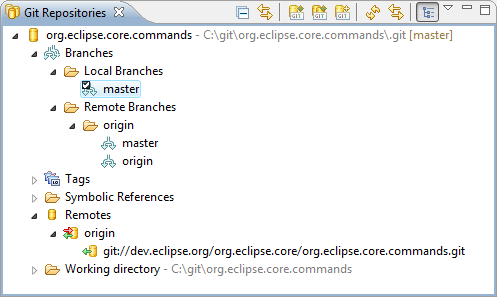
\includegraphics[width=8.4cm]{pics/EGit.png}    % The printed column width is 8.4 cm.
\caption{git repositories presented by EGit / JGit in Eclipse IDE \newline 
screenshot provided by http://eclipse.org/egit/ [2012-01-29]} 
\label{fig:JGit}
\end{center}
\end{figure}

Besides different, mostly platform dependent tools, 
SmartGit represents a current and very functional GUI, which
is available on all popular operating system. Although SmartGit is sold commercially,
a free version for non-commercial projects offered.

Additionally RStudio, a quite new development environment for R supports git (and subversion)
directly since January 2012.


\subsection{git init \& clone}
Now the local git repository can be set up by invoking the
command line command \textit{\lstinline!git init!}. The \textit{\lstinline!git clone!} 
command can be used for creating an exact copy of an available remote repository.

How to clone (copy) the source of this paper, including the whole changelog, to a local folder 
and thereby create a local repository as an exact replica of the online version,
is shown in \verb|line 1| of \textit{Listing \ref{git:clone}}. After the download has
finished, the document can be compiled using the \textit{\lstinline!pdflatex!} command. 

Note that the example in \textit{Listing \ref{git:clone}} shows how to compile 
the \LaTeX file generated by R and Sweave (both are described in chapter \ref{sec:structure}).
It is necessary to run \textit{\lstinline!pdflatex!} two times to produce all references and
listings correctly. 

Although the implementation of the sources takes place on different
linux distributions, the compilation should flawlessly work on other operating systems (OS).
While the tools themself are used in the same way on all popular systems, some details
- like changing the directory using a terminal and setting up the search path to the binaries - may be different.
If the creation of the PDF-file does not work on a specific setup, a prefabricated
version is also located in the git repository. 

\lstset{language=bash,caption={Clone git repository of this paper and compile the included \LaTeX file},label=git:clone,
	morekeywords={git,cd,pdflatex}}
\begin{lstlisting}
git clone git://github.com/FlorianEndel/Mathmod2012.git
cd Mathmod2012
pdflatex Mathmod2012_R_Geospatial_Plotting.tex
pdflatex Mathmod2012_R_Geospatial_Plotting.tex
\end{lstlisting}

After creating a new local git repository or cloning remote sources, everyting is ready for
editing the contents. Git does not anticipate specific software tools like special editors or file browsers. Any file in 
the repository can be edited using any favorite program. Solely the folder (including all contents)
\textit{.git} has to be ignored. Otherwise the local repository may be damaged.

\subsection{git commit, pull, push}
All changes can be permantently 
added to git's history (the changelog) using \textit{\lstinline!git commit!} followed by a 
summary of all changes made (line 1 in listing \ref{git:pullpush_simple}). 
A commited version of the whole project can be restored later on and users are able to
survey all changes over time. This may be
quite useful if something breaks during the implementation of a new feature or adjustment of existing code.
Also try and error approaches may be applied, because resetting a previous state of the whole project is 
quite easy and fast. If the status of the whole project at a specific point in time is necessary, for example
to compare published and updated versions or include comments from a review process, activating  
a previous commit using \textit{\lstinline!git checkout [commit-id]!} may be feasible.

After commiting changes to the \textit{local} repository, it is possible to merge the local version 
with the remote repository (if any exists and is configured) and provide all alterations to other team members or a
public audiance. Before someone pushes the local version to a (central) git server, all changes made
by other people have to be downloaded and included into the own \textit{branch} of the projects source.
Downloading and merging can easily be carried out using \textit{\lstinline!git fetch!} and 
\textit{\lstinline!git merge!}. The command \textit{\lstinline!git pull!} is a combination of
the two previous steps.

If there are no conflicting changes of the source code between the remote and the local
verions, git is normally able to merge everything on its own flawlessly. Sooner or later every team
faces the problem of conflicting and failing merges. The solution for such issues is not straigth forward.
Because the official documentation of git (\url{http://git-scm.com/documentation}) and a quick 
\url{google.com} search may be most helpful, there is no explanation provided within this paper.

Especially during manual merging of conflicting source files, a grphical interface may be very helpful.

Just as the (automatic or manual) marging is finished, it is highly recommended to compile 
the Sweave and \LaTeX file again to be sure that no new errors were introduced. When the merging and
testing procedure is successfully finished, the local changes can be loaded to another remote repository
using \textit{\lstinline!git push!}.

As uploading (pushing) needs the right to write on a remote location, more configuration is normalley 
necessary. As there are serveral possibilities to authenticate to a remote location, 
including different additional tools, signation and encryption, no general explanation can be provided.

The source of this paper is hosted by the free (git) provider \url{github.com}. As shown in 
Listing \ref{git:clone}, it is quite easy to copy (clone) a project from their webservers. 
Uploading (pushing) needs some extra configuration which is explained in the excelent tutorial
provided on \url{help.github.com} (pushing: \url{help.github.com/remotes/#pushing}).

\lstset{language=bash,caption={pull and push of a local git repository without merge conflicts},label=git:pullpush_simple,
	morekeywords={git,cd,pdflatex}}
\begin{lstlisting}
git commit -m 'Summary of changes made'
git pull
pdflatex Mathmod2012_R_Geospatial_Plotting.tex
pdflatex Mathmod2012_R_Geospatial_Plotting.tex
# everything alright?
git push
\end{lstlisting}

\subsection{git: further features}
There are much more useful features of git waiting to be explored and used. Yet again
official documentation on \url{http://git-scm.com/documentation} and practical
tutorials, for example from \url{help.github.com}, are recommended.

In the following listing, the most important 'advanced' features are summarized
(in alphabetical order):
\begin{description}
\item [add] \textit{\lstinline!git add!} is used to add newly created files (within the  folder managed by git) to the current repository.
\item [{branch}] Different branches of the same codebase can be edited independent from
another. In fact, every local clone of a remote repository represents a (remote tracking) 
branch. Branches may be combined using \textit{merge}.
\item [checkout] Switching between different branches (and even create new branches) can
be establiched using \textit{\lstinline!git checkout!}. Even previousely commited versions
can be activated.
\item [log] Using the command \textit{\lstinline!git log!} all prvious commit messages of
the currently activated branch are shown.
\item [{rebase}] Rebase allows to easily change a series of commits, reordering, editing, or squashing commits together into a single commit. It is highly recommended that manipulating the history is performed with great care, because this is one of the rare possibilities to actually loose changes or (under special circumstances) even destroy the repository.
\item [reset] The \textit{\lstinline!git reset!} command is one of the most complicated
functions of git. Be aware that using \textit{reset} is one of the rare
possibilities to actually loose changes! Reseting files or complete (commited) versions
of a branch may be quite useful. A deeper understandig of git's different states -
unstaged, staged, commited - is necessary to effectively use \textit{reset}. A short
and informative introduction to the 'normal workflow' of git can be found here: \url{http://learn.github.com/p/normal.html}.
\item [status] \textit{\lstinline!git status!} shows the status of
the currently activated branch. Most notably new and changed files which may be involved
in the next commit are listed.
\item [tag] Tags are special signs of commited versions. For example a specific revision
of the repository of this paper (listing \ref{git:clone}) is marked (tagged) as published.
\end{description}


\begin{figure}[h]
\begin{center}
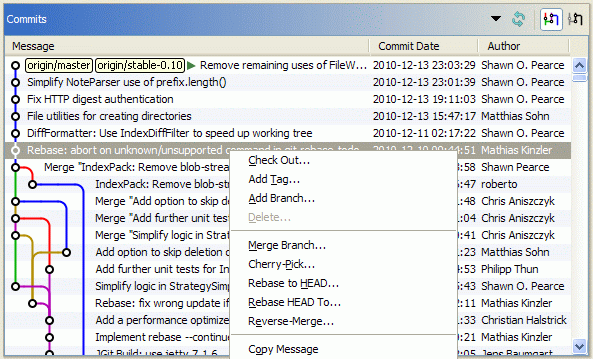
\includegraphics[width=8.4cm]{pics/Smartgit_graphical_Log.png}    % The printed column width is 8.4 cm.
\caption{example for a git changelog and history of commits visualized with Smartgit \newline 
screenshot provided by http://www.syntevo.com/smartgit [2012-01-29]} 
\label{fig:gitHistory}
\end{center}
\end{figure}

\section{\LaTeX, R \& Sweave}\label{sec:structure}

Once the git repository is set up, the Sweave document has to be arranged. 
In the following paragraphs, involved technologies are briefly introduced.

Some central properties are shared by all of them. Availability under a open source license, 
platform independence, multilingualism, lots of documentation and a strong and proofen 
community willing to help are the most important characteristics of these


\subsection{R}
R \citep{R} is known as an upcoming statistical environment. 

As an open source successor of S, it is known to be a powerful and flexible programming language
and computing environment. Especially everyone’s ability to utilize and
contribute to the very rich environment of additional packages hosted 
mainly on “The Comprehensive R Archive Network” are good reasons to give R a try. 
More advanced userRs (spelling “user” and “developer” with capital
’R’s is common in the R community) may use different extensions in 
addition to the variaty of basic packages a normal installation offers.
Most of the more sophisticated packages provide worthwhile 
introductions and even extensive literature. 

R is mainly used by a command line interface. Although this - in comparison
to current graphical user interfaces outdated - way to communicate 
with a computer prgram got a quite steep learning curve, pracitical 
advantages induce many users to learn and stick with it. Mainly the
ease of combining playful exploration of datasets and automatic
reproduction of any steps taken using script- or batch-files are advantageous.

Also the following examples, using special packages providing methods 
for spatial data, may be executed on a simple terminal, a graphical frontend to R,
a remote server or inside a Sweave document. This flexibility enables 
the usage of the same R source code within a database
\footnote{for example \textit{plr} (\url{http://www.joeconway.com/plr/} [2012-01-30]) for PostgreSQL 
\citep{group2011postgresql}}, a local PC and even servers and cloud services.

Of course there are also some graphical user interfaces which may support
the usage of R. The most popular and beginner friendly solutions are
Eclipse with the StatEt plugin and first of all the lately published RStudio
(\url{http://rstudio.org/}). Both are open source and platform independet solution,
which offer many other advantages like project management, integration of version 
management (git), support for Sweave and a client/server separation.

While Eclipse provides considerably more additional plugins and possibilites,
RStudio can be highly recommended to all useRs.

\subsection{Sweave}
Sweave is defined in the official manual \citep{Sweave:Leisch:2002} as follows:
\begin{quotation}
Sweave provides a flexible 
framework for mixing text 
and S code for automatic document generation. 
A single source file contains both documentation text and S code, which are then woven
into a final document
\end{quotation} 

As explained above, R is an open source implementation of S. Therefore both 
language may be interchangeable.

In 2002, Sweave was presented in the former "R Journal"
(\url{http://journal.r-project.org/}) called "R News" (official archive of R News: \url{http://cran.r-project.org/doc/Rnews/}). In the first part of this 
introduction, Sweave is summarized briefely \citep{Sweave:Leisch:2002}:

\begin{quotation}
The purpose of Sweave is to create dynamic reports, 
which can be updated automatically if data or
analysis change. Instead of inserting a prefabricated
graph or table into the report, the master document
contains the R code necessary to obtain it. When run
through R, all data analysis output (tables, graphs, ...) 
is created on the fly and inserted into a final \LaTeX
document. The report can be automatically updated
if data or analysis change, which allows for truly reproducible research.
\end{quotation}

Normally Sweave files got the file extension \texttt{.Rd}. 
After executing \texttt{R CMD Sweave} followed be the filename
of the Sweave document, all R-code is extracted from the document and executed using R.
The results are merged with the \LaTeX code of the \texttt{.Rd} file and saved
to as \texttt{.tex} file with the same filename. Afterwards the common 
compilation using \texttt{latex}, \texttt{pdflatex}, \texttt{bibtex}, and so on
can be performed.

\subsection{simple Sweave document}

This subsection shows the basic structure of a Sweave document. As this
paper is written using \LaTeX and R, another working example can be found
in the git repository, described in Listing \ref{git:clone} on page
\pageref{git:clone}.

At the beginning (line 1 to 5) of Listing \ref{sweave:simple}, a very simple
\LaTeX-Document is shown. On line 6 an R-environment is declared using 
the "noweb" syntax, which is described in \cite{Ramsey_1994, Johnson_Johnson_2000}.
Between \newline \texttt{<<label1, echo=false, results=hide>>=} \newline and the
@-sign, R source code can be located. In the header of the environment are
some (local) settings an the name, which is displayed during the
compilation process, located. The \textit{results} setting defines how
output generated by R should be handled by the \LaTeX processor and \textit{echo}
configures wether messages from R should be included in the output.

More details about configuration of the noweb-environment of Sweave can
be found in the official manual \citep{SweaveManual}.

Some additional functionalities are shown in the example. In addition to the
whole declaration, any appearance of \texttt{\textbackslash{}Sexpr\{\#R-Code\}}
is also exected by R an any output is included in the document. This may be
quite useful if single values of an calculation should be inserted into 
continous text.

\texttt{\textbackslash{}SweaveInput\{filename\}} can be used to include 
another Sweave file. Although importing additional souce code can be realized with
R, partitioning a document to several Sweave files may be handy.

All single R environments which are executed in the same process share one
global namespace. Also libraries, like \texttt{xtable} (loaded on line 7), which eases the
creation of \LaTeX tables out of data stored in R, are
available throughout the document.


\lstset{language=Octave,caption={basic structure of a Sweave document},label=sweave:simple}
\begin{lstlisting}
\documentclass[a4paper]{article}
% additional \LaTeX configuration

\begin{document}

<<label1, echo=false, results=hide>>=
library(xtable)
# R code following
@

<<LaTex_Output, echo=hide, results=tex>>=
# R code generating \LaTeX
@

<<>>=
# empty header, standard settings
@

Normal \LaTeX code and a single line from \Sexpr{print('R')}.

\SweaveInput{./includes/config}


\end{document}
\end{lstlisting}

\section{Geospatial Plotting}

Finally the most important preparations are ready and some geospatial plots 
generated using R can be shown. 

\section{Conclusion}


\bibliography{lit}   

\end{document}
